\selectlanguage{german}
\subsection{YOLOv5}
\nameref{subsec:yolo}, ein Bilderkennungsmodell, wurde von Joseph Redmon und Ali Farhadi an der Universität von Washington entwickelt und im Jahr 2015 veröffentlicht. \nameref{subsec:yolo} steht für "You Only Look Once", was darauf hinweist, dass das Modell nur einmal auf ein Bild schaut, um Objekte schnell und präzise zu erkennen. Seit seiner Veröffentlichung wurden insgesamt neun Versionen von \nameref{subsec:yolo} veröffentlicht \cite{Yolo} .

\subsubsection{Das Modell}
Ein vortrainiertes Modell der fünften Version von \nameref{subsec:yolo} wird verwendet, welches bereits spezifisch für die gegebenen Anforderungen trainiert ist. Obwohl es sich um eine ältere Version von YOLO handelt, ist die Effektivität des Modells nicht beeinträchtigt. YOLOv5 zeigt gerade bei begrenzten Hardware-Ressourcen wie dem Raspberry Pi 4 eine höhere Geschwindigkeit im Vergleich zu neueren Versionen wie YOLOv8. Vorteilhaft ist auch, dass eine kleinere Variante von \nameref{subsec:yolo}, nämlich Yolov5s, genutzt wird. Dieses Modell wurde mit Bildern aus diversen Quellen trainiert, wobei ein benutzerdefiniertes Datenset aus 374 Trainingsbildern und 111 Validierungsbildern erstellt wurde.

\subsubsection{Makesense.ai}
Für das Labeln der Daten kommt Makesense.ai zum Einsatz, eine Plattform, die es Nutzern erlaubt, Bilder hochzuladen und mit Annotationen wie Bounding Boxes und Klassifizierungen zu versehen. Dies dient der Vorbereitung von Datensätzen für Anwendungen in der Computer Vision \cite{noauthor_make_nodate}. Die Daten sind dabei in drei Klassen untergliedert: 'walking', 'sitting' und 'fall detected' (siehe Abbildung \ref{fig:yolo_classes}).


\begin{figure}[H]
	\centering
	\begin{minipage}[b]{0.3\textwidth}
		\centering
		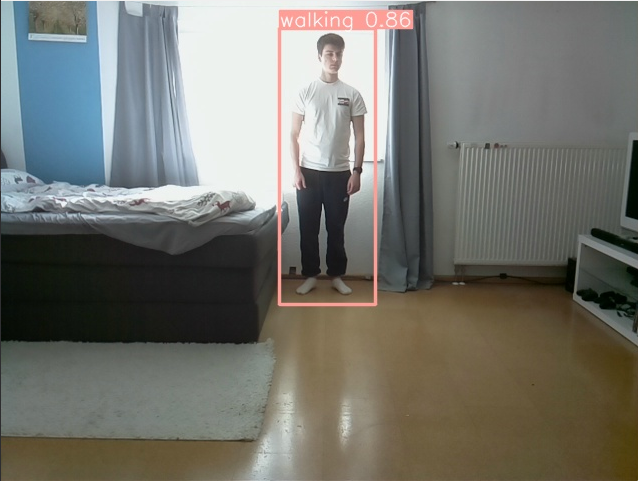
\includegraphics[width=\textwidth]{images/walking.png}
		\caption*{Klasse: ''walking''}
	\end{minipage}
	\hfill
	\begin{minipage}[b]{0.3\textwidth}
		\centering
		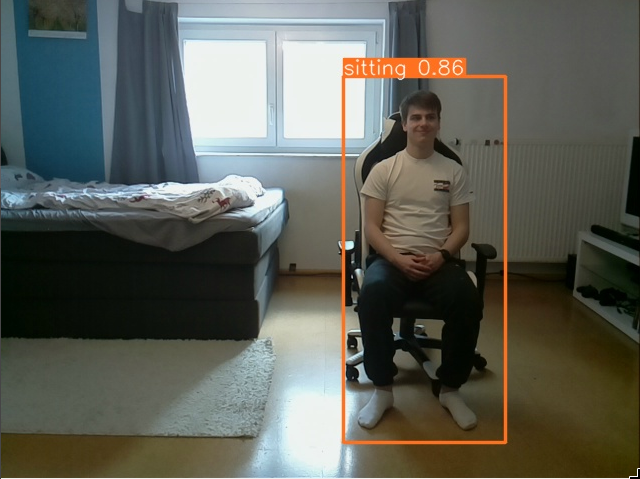
\includegraphics[width=\textwidth]{images/sitting.png}
		\caption*{Klasse: ''sitting''}
	\end{minipage}
	\hfill
	\begin{minipage}[b]{0.3\textwidth}
		\centering
		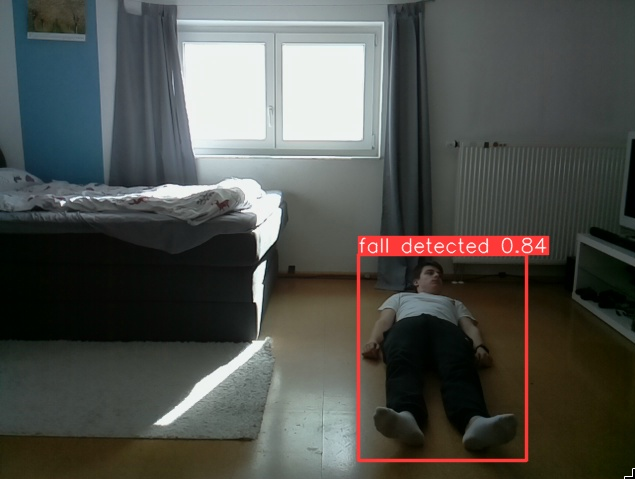
\includegraphics[width=\textwidth]{images/fallen.png}
		\caption*{Klasse: ''fall detected''}
	\end{minipage}
	\caption{YOLOv5 Detektion Klassen}
	\label{fig:yolo_classes}
\end{figure}



\subsubsection{Anbindung}
Die Anbindung an das YOLOv5-Modell erfolgt über PyTorch, ein Open-Source-Framework für maschinelles Lernen, das auf der Programmiersprache Python und der Torch-Bibliothek basiert. PyTorch wurde 2016 von einem Forscherteam für künstliche Intelligenz bei Facebook entwickelt \cite{noauthor_pytorch_nodate}.

Das Modell läuft in einem Docker-\nameref{subsec:container}, der kontinuierlich über MQTT einen int-Wert veröffentlicht, um anzuzeigen, ob der Zustand  \nameref{subsec:normal},   \nameref{subsec:warnung} oder  \nameref{subsec:alarm} aufgetreten ist. Zur Einbindung der Raspberry Pi Kamera verwendet der \nameref{subsec:container} auch OpenCV, eine Open-Source-Bibliothek für Computer Vision \cite{OpenCV}. Mithilfe von OpenCV wird auch eine Funktion entwickelt, die über \nameref{subsec:mqtt} ein Bild mit allen Detektionen versendet. Diese Bilder werden später mithilfe eines weiteren \nameref{subsec:docker} Containers auf einem lokalen Rechner angezeigt.



% Zitat von wo das 85% bis 90% genauigkeit ist. Quelle fehlt, noch ergänzen.
